\title{Operating Systems–2: CS3523 2019\\
Programming Assignment 3: \\
Solving Producer Consumer Problem using\\
Semaphores and Locks\\
Report}
\author{Sai Harsha Kottapalli\\CS17BTECH11036}
\date{March 8, 2019}

\documentclass[12pt]{article}
\usepackage{graphicx}

\begin{document}
\maketitle

\section{Aim}
The goal of this assignment is to solve the bounded buffer producer-consumer problem using Semaphores and Locks
in C++.

\section{Design of the Program :}
We use Locks and Semaphores to implement the bounded buffer producer-consumer problem.
\subsection{Critical Section :}
This part of the code should be accessed by only one producer/consumer respectively at a time or as an atomic equivalent.
We can avoid race conditions by making sure that no two producers/consumers enter their Critical Sections at the same time.
\subsection{Entry Section :}
This part of the code is accessible for all the producers/consumers. The job of this code is to make sure only one producer/consumer is given access to the critical section at a particular time.
\subsection{Exit Section :}
This part of the code is where the producer/consumer has successfully executed the critical section of the program, and will reset the lock so that other producers/consumers can now enter the critical section(if any) while this producer/consumer completes the remainder section parallelly.
\subsection{Average Waiting Time :}
This is defined as the amount of time each access to critical section takes after requesting for the same.
\subsection{Buffer section :}
The producer and consumer which are currently in their respective critical section access buffer section such that only one of them is inside this section and in case the (producer tries to produce)/(consumer tries to consume) from buffer when it is full/empty, it gives the access of buffer to the other.

\section{Explanation of program - Common Part}

\subsection{Header files used}
\begin{itemize}
\item \textbf{iostream}\\
Header that defines the standard input/output stream objects
\item \textbf{thread}\\
Used for implementing threads.\\
It defines the class to represent individual threads of execution.\\
A thread of execution is a sequence of instructions that can be executed concurrently with other such sequences in multithreading environments, while sharing a same address space.\\
\item \textbf{fstream}\\
Input/output stream class to operate on files.
\item \textbf{random}\\
This header introduces random number generation facilities.\\
\item \textbf{cstdio}\\
Used for \textbf{sprintf}, that is, for the format in which the time has to be printed to the log file.
\item \textbf{unistd.h}\\
Used for miscellaneous symbolic constants and types, and declares miscellaneous functions - \\
\textbf{localtime} - which is used to get a structure of time, with hours, minutes and seconds.\\
\textbf{time} - For capturing current time which is processed by above command.
\item \textbf{string}\\
For processing strings.
\item \textbf{sys/time.h}\\
For using \textbf{gettimeofday()} to obtain the time a producer/consumer has to wait to get access through the lock or semaphore.
\end{itemize}

\subsection{getInput()}
This is a helper function which helps in keeping the code modular.\\
It reads the value of the following from the input file, specified in ReadMe.txt \\
\begin{itemize}
\item Capacity of the buffer
\item Number of Producers - n$\textunderscore$p\\
\item Number of Consumers - $\textunderscore$c\
\item Number of times each producer should produce - rep$\textunderscore$p\\
\item Number of times each consumer should consume - rep$\textunderscore$c\\
\item lam1 and lam2\\
Represents the mean of value of two exponential distribution curves which is to be constructed.
\end{itemize}

\subsection{producer()}
The producer function is responsible to produce data for the consumption of consumer.\\
The producer won't try to add data into the buffer if it's full.

\subsection{consumer()}
The consumer function is responsible to consume data produced by producer.\\
The consumer won't try to remove data from the buffer if it's empty.

\subsection{currTime()}
Takes input time$\textunderscore$t structure to generate the time in HH:MM:SS syntax and return this as a string.

\subsection{Buffer}
We use circular queue to implement the buffer for the producer/consumer problem.

\subsection{Other important variables used}
\begin{itemize}
\item \textbf{exponential$\textunderscore$distribution}\\
Produces random non-negative floating-point values x, distributed according to probability density function defined for exponential distribution about the constant rate given as a parameter.
\item \textbf{default$\textunderscore$random$\textunderscore$engine}\\
This is a random number engine class that generates pseudo-random numbers.
\item \textbf{buffer}\\
Dynamic array of bool type, based on capacity given in input file.
\item \textbf{thread *th for producers and consumers}\\
th$\textunderscore$p and th$\textunderscore$c are the pointers for storing the array of n$\textunderscore$p and n$\textunderscore$c threads respectively. This will be useful for later calling join to properly exit the threads spawned previously.
\item \textbf{waiting time for producers and consumers}
Used to calculate the average time a producer/consumer has to wait to get access through locks or semaphores.
\end{itemize}

\section{Locks}
A lock or mutex (from mutual exclusion) is a synchronization mechanism for enforcing limits on access to a resource in an environment where there are many threads of execution. A lock is designed to enforce a mutual exclusion concurrency control policy.\\
Header file used - \textbf{mutex}\\
The following functions of semaphore in c is  utilized to solve the current problem - \\
\begin{itemize}
\item \textbf{mutex::lock}
If the mutex isn't currently locked by any thread, the calling thread locks it (from this point, and until its member unlock is called, the thread owns the mutex).\\
If the mutex is currently locked by another thread, execution of the calling thread is blocked until unlocked by the other thread (other non-locked threads continue their execution).\\
If the mutex is currently locked by the same thread calling this function, it produces a deadlock (with undefined behavior).\\
\item \textbf{mutex::unlock}
Unlocks the mutex, releasing ownership over it.\\
If the mutex is not currently locked by the calling thread, it causes undefined behavior.
\end{itemize}

\section{Semaphores}
A semaphore is a variable or abstract data type used to control access to a common resource by multiple processes in a concurrent system such as a multitasking operating system. A semaphore is simply a variable. This variable is used to solve critical section problems and to achieve process synchronization in the multi processing environment.\\
Header file used - \textbf{semaphore.h}\\
The following functions of semaphore in c is  utilized to solve the current problem - 
\begin{itemize}
\item \textbf{sem$\textunderscore$init(sem$\textunderscore$t *sem, int pshared, unsigned int value);}\\
Initializes the unnamed semaphore at the address pointed
to by sem.  The value argument specifies the initial value for the
semaphore.\\
The pshared argument indicates whether this semaphore is to be shared
between the threads of a process, or between processes.
\item \textbf{sem$\textunderscore$wait(sem$\textunderscore$ t *sem);}\\
decrements (locks) the semaphore pointed to by sem.  If
the semaphore's value is greater than zero, then the decrement
proceeds, and the function returns, immediately.  If the semaphore
currently has the value zero, then the call blocks until either it
becomes possible to perform the decrement (i.e., the semaphore value
rises above zero), or a signal handler interrupts the call.
\item \textbf{sem$\textunderscore$post(sem$\textunderscore$t *sem);}\\
increments (unlocks) the semaphore pointed to by sem.  If
the semaphore's value consequently becomes greater than zero, then
another process or thread blocked in a sem$\textunderscore$wait() call will be woken
up and proceed to lock the semaphore.
\item \textbf{sem$\textunderscore$destroy(sem$\textunderscore$t *sem);}\\
destroys the unnamed semaphore at the address pointed to by sem.
\item We use "full" and "empty" semaphores, initialized to 0 and buffer$\textunderscore$size respectively for producers and consumers while a binary semaphore for the buffer.
\end{itemize}

\pagebreak

\section{Comparision}
\subsection{Graphs}
\begin{figure}[ht!]
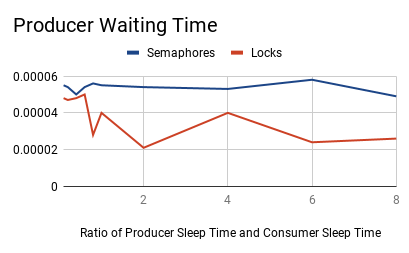
\includegraphics[width=150mm]{Producer_Waiting_Time.png}
\caption{Comparision between Average time taken for accessing the critical section by producers to produce data using locks and semaphores}
\end{figure}
\begin{figure}[ht!]
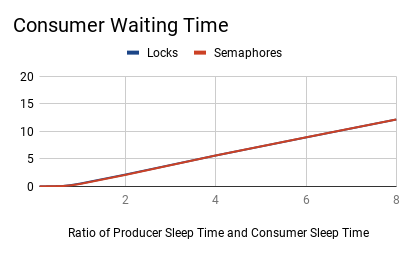
\includegraphics[width=150mm]{Consumer_Waiting_Time.png}
\caption{Comparision between Average time taken for accessing the critical section by consumer to consume data using locks and semaphores}
\end{figure}
\pagebreak
\subsection{Notes}
\begin{itemize}
\item Parameters used for test cases:\\
capacity = 100\\
n$\textunderscore$p = 10\\
n$\textunderscore$c = 15\\
rep$\textunderscore$p = 15\\
rep$\textunderscore$c = 10\\
$\Lambda _1$ = a seconds and $\Lambda _2$ = b seconds, such that,\\
a + b = 20 and a/b = 10, 8, 6, 4, 2, 1, 0.8, 0.6, 0.4, 0.2, 0.1.
\item Each of the plotted points is the average of 5 testcases.\\
\item Locks perform better than semaphores.
\item Sleep and wakeup calls are genarally more expensive.
\item When buffer is small, usage of locks is suggested because busy waiting seems better than sleep and wakeup.
\item CPU usage is very high when locks are used when compared to that of semaphores.\\
This is because of busy-waiting in case of locks as opposed to sleep and wakeup in semaphores.
\item 
\end{itemize}

\end{document}